\documentclass[12pt]{article}
\usepackage[utf8]{inputenc}
\usepackage[T1]{fontenc}
\usepackage{pdflscape} 
\usepackage{lmodern}
\usepackage{amsmath}
\usepackage[a4paper,bindingoffset=0.2in,%
            left=0.5in,right=0.5in,top=0.5in,bottom=1in,%
            footskip=.25in]{geometry}
\usepackage[colorlinks=true, linkcolor=Black, urlcolor=Blue]{hyperref}
\usepackage{graphicx}
\usepackage{subcaption}
\usepackage{listings}
\usepackage{color}
\usepackage{float}
\usepackage[usenames, dvipsnames]{xcolor}

\definecolor{codegreen}{rgb}{0,0.6,0}
\definecolor{codegray}{rgb}{0.5,0.5,0.5}
\definecolor{codepurple}{rgb}{0.58,0,0.82}
\definecolor{backcolour}{rgb}{0.95,0.95,0.92}

\lstdefinestyle{mystyle}{
	backgroundcolor=\color{backcolour},   
	commentstyle=\color{codegreen},
	keywordstyle=\color{magenta},
	numberstyle=\tiny\color{codegray},
	stringstyle=\color{codepurple},
	basicstyle=\ttfamily\footnotesize,
	breakatwhitespace=false,         
	breaklines=true,                 
	captionpos=b,                    
	keepspaces=true,                 
	numbers=left,                    
	numbersep=5pt,                  
	showspaces=false,                
	showstringspaces=false,
	showtabs=false,                  
	tabsize=2
}


\begin{document}
\title{Projekt 2: Analiza możliwości algorytmów optymalizacji\\
\large Sebastian Michoń 136770, Marcin Zatorski 136834\\
\large grupa L5}
\date{\vspace{-10ex}}
\maketitle

\section{Zarys idei}
\begin{enumerate}
	\item Obliczenia przeprowadzano dla 2 architekur:
	\begin{enumerate}
		\item Standardowa sieć neuronowa, złożona z warstw gęstych o kolejno 10-50(sigmoid)-100(sigmoid)-100(relu)-100(tanh)-5(sigmoid) neuronach (10 neuronów wejściowych, 5 wyjściowych; w nawiasach podano funkcje aktywacji).
		\item Konwolucyjna sieć neuronowa, złożona z 2 kolejnych warstw konwolucyjnych i max poolingu (conv2d(relu)-max\_pool-conv2d(relu)-max\_pool-flatten) a następnie 3 warstw gęstych o kolejno 100(sigmoid)-100(sigmoid)-5(sigmoid) neuronach. Przyjmuje na wejście tablicę trójwymiarową o rozmiarach 10x10x3
	\end{enumerate}

	\item Operacje przeprowadzone dla pierwszej architektury:
	\begin{enumerate}
		\item Stworzono pewną sieć neuronową, dane treningowe i dane testowe. Dane treningowe składały się z 50.000 instancji, dane testowe z 10.000 instancji (instancje składały się z 10 wartości). Dane pochodziły z rozkładu normalnego.
		\item Uruchamiano losowo zainicjalizowaną (z biasem z rozkładu normalnego i wagami pochodzącymi z jednorodnego inicjalizatora Xaviera) sieć neuronową dla danych treningowych. Będzie ona nazywana dalej prewzorcową siecią neuronową.
		\item W każdym pojedynczym eksperymencie porównywano określone optymalizatory w następujący sposób:
		\begin{enumerate}
			\item Ustalano ground truth jako rezultat propagacji zestawu treningowego i testowego przez sieć neuronową z wagami pochodzącymi z prewzorcowej sieci neuronowej i regularyzacją (gdyby używać prewzorcowej sieci neuronowej z takimi samymi wagami i bez regularyzacji, wyniki mogłyby się różnić dla regularyzacji 'batch  normalization'; Dzięki rozwiązaniu zadania w taki sposób spełniono założenie o identycznej architekturze sieci neuronowych jednocześnie - dzięki kopiowaniu wag - umożliwiając porównywanie rezultatów dla różnych rodzajów regularyzacji). Sieć ta nazywana będzie wzorcową siecią neuronową.
			\item Tworzono sieć neuronową dla podanej metody regularyzacji i podanych hiperparametrów (np. $dropout\_rate=0.2$). Nazywana ona będzie dalej testową siecią neuronową.
			\item Trenowano testową sieć neuronową w 3 epokach, domyślnie dla $batch\_size=32$ z podanym optymalizatorem.
			\item Po wytrenowaniu testowej sieci neuronowej ewaluowano ją na zbiorze treningowym, testowym i porównywano wagi w dwóch sieciach neuronowych: testowej i wzorcowej.
			\item Kroki od 2. wykonywano dla pozostałych optymalizatorów.	
		\end{enumerate}
	\end{enumerate}
	\item Dla drugiej w analogiczny sposób przeprowadzono następujące operacje:
	\begin{enumerate}
		\item Stworzono pewną sieć neuronową, dane treningowe i dane testowe. Dane treningowe składały się z 20.000 instancji, dane testowe z 5.000 instancji (instancje składały się z trójwymiarowej macierzy o rozmiarach 10x10x3). Dane pochodziły z rozkładu jednostajnego.
		
		\item Uruchamiano losowo zainicjalizowaną (z biasem z rozkładu normalnego dla warstw gęstych, biasem zainicjalizowanym zerami dla warstw konwolucyjnych i wagami pochodzącymi z jednorodnego inicjalizatora Xaviera zarówno dla warstw gęstych, jak i konwolucyjnych) sieć neuronową dla danych treningowych. Będzie ona nazywana dalej prewzorcową siecią neuronową.
		\item Pojedynczy eksperyment był identyczny jak w przypadku klasycznej sieci neuronowej.
	\end{enumerate}
	\item Funkcją kosztu dla porównania danych wyjściowych z testowej sieci do danych ground truth było MSE.
	\item Dla pierwszej i drugiej architektury eksperymenty przeprowadzono dla następujących typów regularyzacji:
	\begin{enumerate}
		\item \textbf{batch\_normalization}: przeprowadzano testy dla 3 optymalizatorów: SGD, Adam i AdamW(weight\_decay = 0.0001). Przeprowadzono testy dla każdej pary złożonej z wartości z ciągu [4, 16, 64, 256] dla parametru batch\_size i wartości z ciągu [0.1, 0.5, 0.9, 0.95, 0.99, 0.999] dla parametru momentum - w sumie wykonano 24 eksperymenty dla tej regularyzacji.
		
		\item \textbf{weight\_decay}: przeprowadzano testy dla 2 optymalizatorów: SGDW i AdamW. Przeprowadzono testy dla każdej wartości z ciągu [0.5, 0.1, 0.01, 0.001, 0.0001, 0.00001] dla parametru weight\_decay - w sumie wykonano 6 eksperymentów dla tej regularyzacji.
		
		\item \textbf{dropout}: przeprowadzano testy dla 3 optymalizatorów: SGD, Adam i AdamW(weight\_decay = 0.0001). Przeprowadzono testy dla każdej wartości z ciągu [0, 0.1, 0.2, 0.3, 0.4, 0.5] dla parametru dropout\_rate - w sumie wykonano 6 eksperymentów dla tej regularyzacji.
	\end{enumerate}
	Wykonano zatem w sumie 36 eksperymentów. Zbiór takich 36 eksperymentów nazywany będzie dalej pełnym testem. Dla standardowej sieci wartwy Dropout / Batch normalization wstawiono pomiędzy każdą parę warstw gęstych z wyłączeniem pierwszych 2 warstw (czyli na przykład 10-50-Dropout-100-Dropout-100-Dropout-100-Dropout-5).
	Dla sieci konwolucyjnej wstawiano wartwy dropout i batch normalization w te same miejsca, ponadto:
	\begin{enumerate}
		\item Za warstwą konwolucyjną wstawiono dropout.
		\item Za warstwą max\_pooling wstawiono batch\_normalization, jeśli właśnie ten typ regularyzacji był testowany.
	\end{enumerate}	
	
	\item \label{tit:cost} Funkcja kosztu wag dla standardowej sieci gęstej:
	\begin{enumerate}
		\item Zaimplementowano standardową funkcję liczącą MSE będącą uśrednioną sumą błędów kwadratowych dla wszystkich wag i biasów (bias liczony był w średniej MSE jako jedna z wag).
		\item Aby porównywać wagi neuronów, które są w jakiś sposób związane, przed wyliczeniem funkcji kosztu modyfikowano macierze wag w wytrenowanej testowej sieci neuronowej tak, aby neurony, które mają podobne wartości wag i biasa na wejściu były na tych samych pozycjach w obydwu porównywanych sieciach neuronowych.
		\item W \textit{tensorflow} element macierzy wag $W_{i,j}$ oznacza wagę $i$-tego wyjścia z poprzedniej warstwy dla $j$-tego wejścia kolejnej warstwy. Co za tym idzie, wektor $V_j=[W_{1,j}, W_{2,j} \dots W_{n,j}, b_j]$ reprezentuje kolejne wagi na wejściu $j$-tego neurona w kolejnej warstwie.
		\item Dla wszystkich macierzy wag i biasów - począwszy od pierwszej - porównywano ujemne podobieństwo kosinusowe pomiędzy każdą parą wektorów $V_j$ w obu sieciach (wzorcowej i testowej) dla tej samej warstwy.
		\item Celem metody była maksymalizacja podobieństwa neuronów na tych samych pozycjach; w tym celu wykorzystano metodę węgierską, aby wybrać minimalną możliwą sumę ujemnych podobieństw kosinusowych przy pewnej zamianie miejscami pozycji neuronów. Rezultatem metody węgierskiej była sekwencja par $1:a_1, 2:a_2, \dots m:a_m$ oznaczająca, że aby zminimalizować sumę ujemnych podobieństw kosinusowych wektorów wag (z biasem) dla pojedynczego neurona należy dokonać takiej transformacji na macierzy wag, aby kolumna o indeksie $a_i$ była na pozycji \(i\)-tej po transformacji testowej sieci neuronowej. Transormację tę osiągnięto przez:
		$$\begin{bmatrix}
			k_1 & k_2 \dots k_m\\
		\end{bmatrix}
		\begin{bmatrix}
			e_{a_1} & e_{a_2} & \dots e_{a_m}\\
		\end{bmatrix}
		=
		\begin{bmatrix}
			k'_1 & k'_2 & \dots k'_m\\
		\end{bmatrix}
		$$
		gdzie \(e_i\) oznacza pionowy wektor jednostkowy wypełniony zerami i jedną jedynką w pozycji \(i\)-tej, wektory jednostkowe mają rozmiar \(m\) (macierz z prawej jest kwadratowa), wektory \(k_j\) to kolumny macierzy wag przed transformacją. W ten sam sposób transformowano wektor biasów.
		\item Analogicznie, jeśli za daną warstwą była inna wartswa gęsta, zamieniono kolejnością wiersze następnej macierzy wag tak, aby kolejność neuronów była taka sama w obu macierzach (a zatem należało zmienić kolejność wartości wychodzących z poprzedniej warstwy):
		$$\begin{bmatrix}
			e_{a_1}^T\\ e_{a_2}^T\\ \dots\\ e_{a_m}^T\\
		\end{bmatrix}
		\begin{bmatrix}
			w_1\\ w_2\\ \dots\\ w_m\\
		\end{bmatrix}
		=
		\begin{bmatrix}
			w'_1\\ w'_2\\ \dots\\ w'_m\\
		\end{bmatrix}
		$$ gdzie $w_i$ oznacza $i$-ty wiersz pierwotnej macierzy. Nie transformowano wektora biasów, ponieważ nie miał on związku z transformacją pozycji wyjść z poprzedniej warstwy.
	\end{enumerate}
	\item \label{tit:cost_cnn} Funkcja kosztu wag dla sieci konwolucyjnej była standardową funkcją opisaną w skrypcie projektu: MSE pomiędzy wszytkimi wagami i biasami w obu sieciach, funkcja ta nie bierze pod uwagę permutacji neuronów; powodów odstąpienia od opisanej wyżej funkcji kosztu dla wag było kilka:
	\begin{enumerate}
		\item Jest ona powolna; Przetwarzanie wszystkich opisanych powyżej testów w 3 epokach trwało ok. 2h. Aby ją przyspieszyć, najpewniej należałoby wykonać pewne operacje na poziomie Cythona (złożonościowo $O(n^3)$ nie jest problemem, operacje na pojedynczych elementach macierzy tensorflow - już tak).
		\item Po kilku warstwach wartości MSE wynikające z porównania macierzy wag bez uwzględniania permutacji były bardzo podobne dla algorytmu opisanego w punkcie \ref{tit:cost}; wynika to m.in. z propagacji błędu (metoda opisana wyżej ma sens, jeśli neurony we wcześniejszej warstwie są w prawie takiej samej kolejności w testowej i wzorcowej sieci neuronowej; liczba błędnie weryfikowanych neuronów rosła wraz z każdą warstwą do momentu, w którym funkcje kosztu dla obu metod po ~5 warstwach były nieomal identyczne).
	\end{enumerate}
	\item Przeprowadzono 5 pełnych testów, opisano w tym sprawozdaniu tylko 2. Pozostałe zostały pokrótce opisane w podrozdziale \ref{tit:testo}, wykresy pochodzące z tych eksperymentów znajdują się w folderze \textit{Comparisions}.

\end{enumerate}
\section{Rezultaty i ich omówienie}
\subsection{Testy pierwszej sieci}\label{tit:ann}
\subsubsection{Testy batch normalization}
\begin{figure}[h!]
	\centering
	\begin{subfigure}[b]{1\linewidth}
		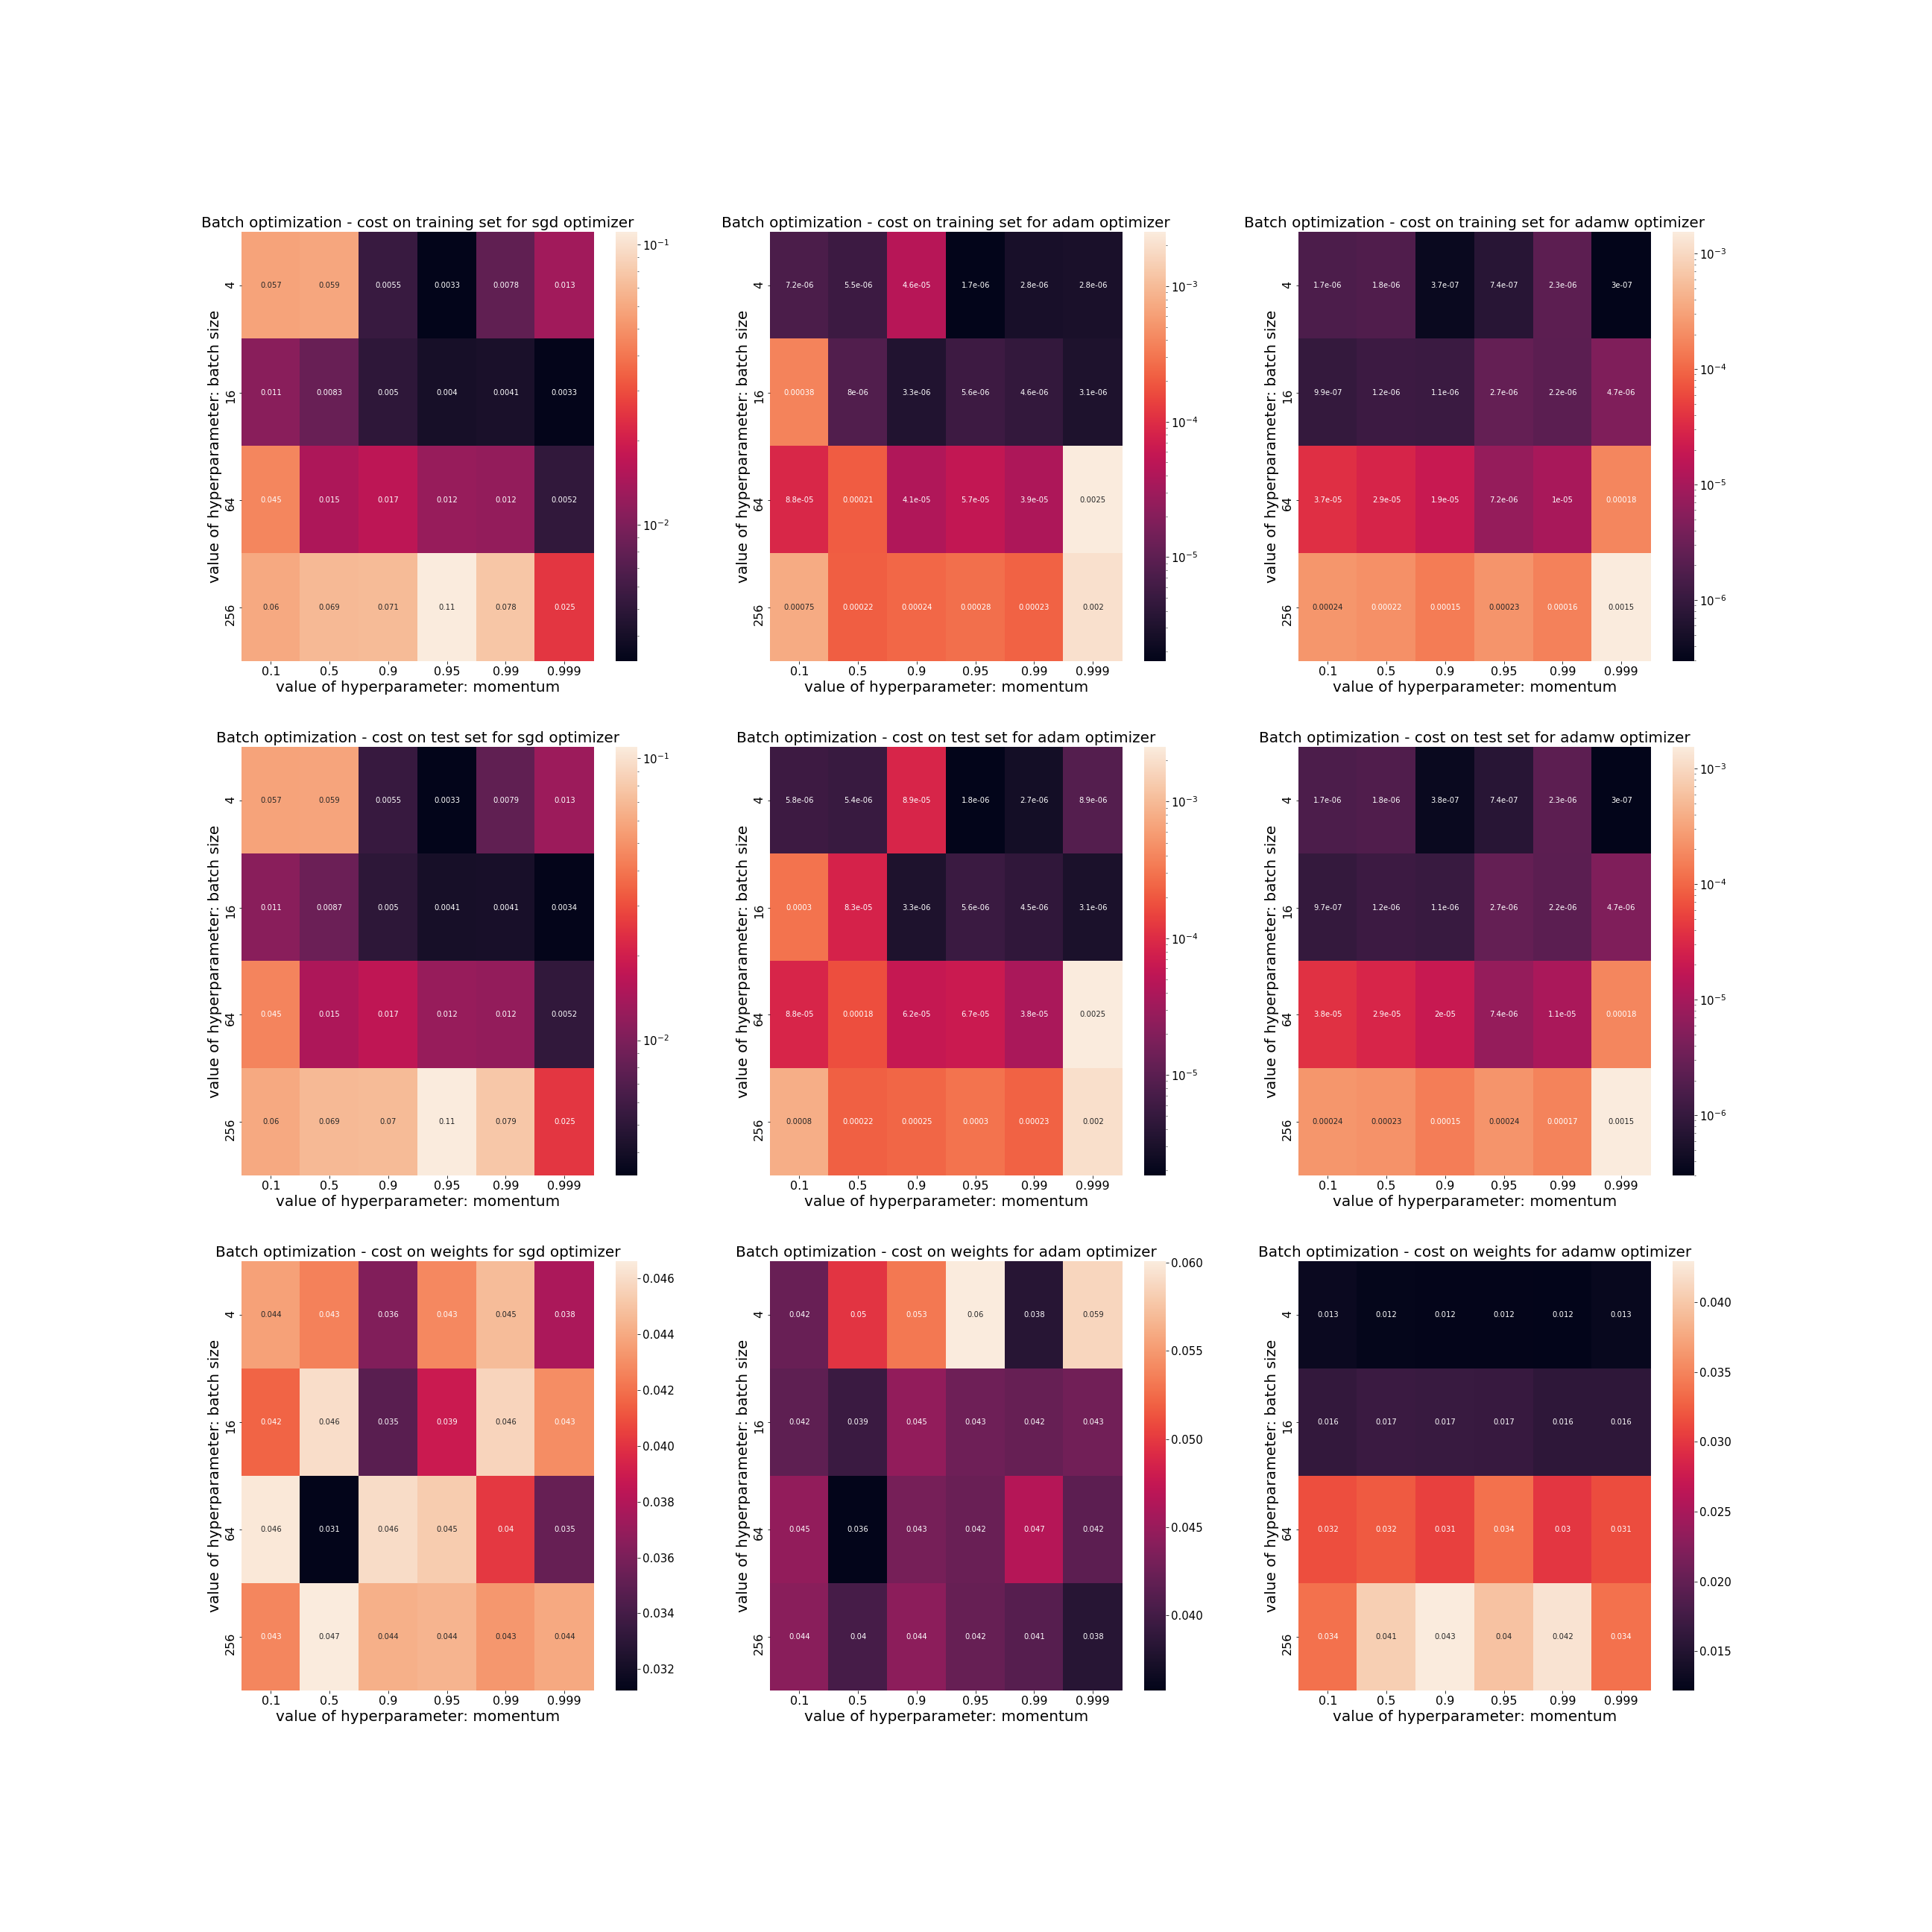
\includegraphics[width=\linewidth]{Comparision_batch_norm_ann_0.png}
	\end{subfigure}
	\caption{Rezultaty nauki sieci z regularyzacją typu batch normalization}
	\label{fig:batch_ann}
\end{figure}
Opis testów i ich rezultatów:
\begin{enumerate}
	\item Na tym i każdym kolejnym wykresie wartości funkcji kosztu dla zestawu testowego i treningowego będą przedstawiane w skali logarytmicznej, nawet dla SGD.
	\item Funkcja kosztu dla zbioru treningowego i testowego to MSE z porównania outputów sieci testowej i sieci wzorcowej, dla wag jest to wartość wyznaczona w sposób opisany w punkcie \ref{tit:cost} (rozdział 1.).
	\item Wartości funkcji kosztu dla zbioru treningowego i testowego są nieomal identyczne - wynika to z:
	\begin{enumerate}
		\item 50.000 Instancji danych treningowych pochodzących z tego samego rozkładu co dane testowe - pociąga to za sobą możliwość efektywnego wytrenowania sieci.
		\item Braku szumu w danych wyjściowych - Wzorcowe wartości na wyjściu są funkcją zależną jedynie od inputu.
		\item Identycznej architektury obu sieci neuronowych.
	\end{enumerate}
	Obserwacja ta będzie zauważalna we wszystkich kolejnych testach.
	\item Najlepsze rezultaty optymalizatora SGD dla zbioru treningowego i testowego w tych eksperymentach (wartość MSE rzędu około 0.001) są porównywalne z najgorszymi rezultatami optymalizacji Adam i AdamW. Obserwacja ta będzie się powtarzała w kolejnych testach.
	\item Wszystkie optymalizatory uzyskały najniższe wartości funkcji kosztu dla zbioru treningowego i testowego dla momentum=0.95 albo 0.9 (w teście ann\_1 tej architektury najlepszą wartością momentum było zawsze 0.99).
	\item Dla SGD najlepsze i najbardziej stabilne wartości funkcji kosztu dla zbioru treningowego i testowego osiągano dla $batch\_size=16$, dla Adam i AdamW dla $batch\_size=4$.
	\item Wartości fukcji kosztu dla zbioru treningowego i testowego dla batch\_size wyższego równego 64 są prawie zawsze wyższe niż dla mniejszego batch\_size (przy czym im wyższy batch\_size, tym szybciej wykonują się obliczenia).
	\item AdamW dla $batch\_size=4$ bardzo dobrze dopasowywał się do wag sieci wzorcowej; żaden inny optymalizator w tym eksperymencie nie osiągnął podobnych rezultatów dla opisanej w paragrafie \ref{tit:cost} funkcji kosztu (0.12 AdamW względem 0.31 SGD). W ogólności AdamW lepiej dopasowywał wagi do sieci wzorcowej niż pozostałe optymalizatory zarówno w tych eksperymentach, jak i w następnych.
	\item Wagi sieci neuronowej będące rezultatem optymalizacji SGD są bardziej zbliżone do wag wzorcowej sieci neuronowej niż wagi będące rezultatem optymalizacji algorytmem Adam.
\end{enumerate}

\subsubsection{Testy weight decay}
\begin{figure}[H]
	\centering
	\begin{subfigure}[b]{1\linewidth}
		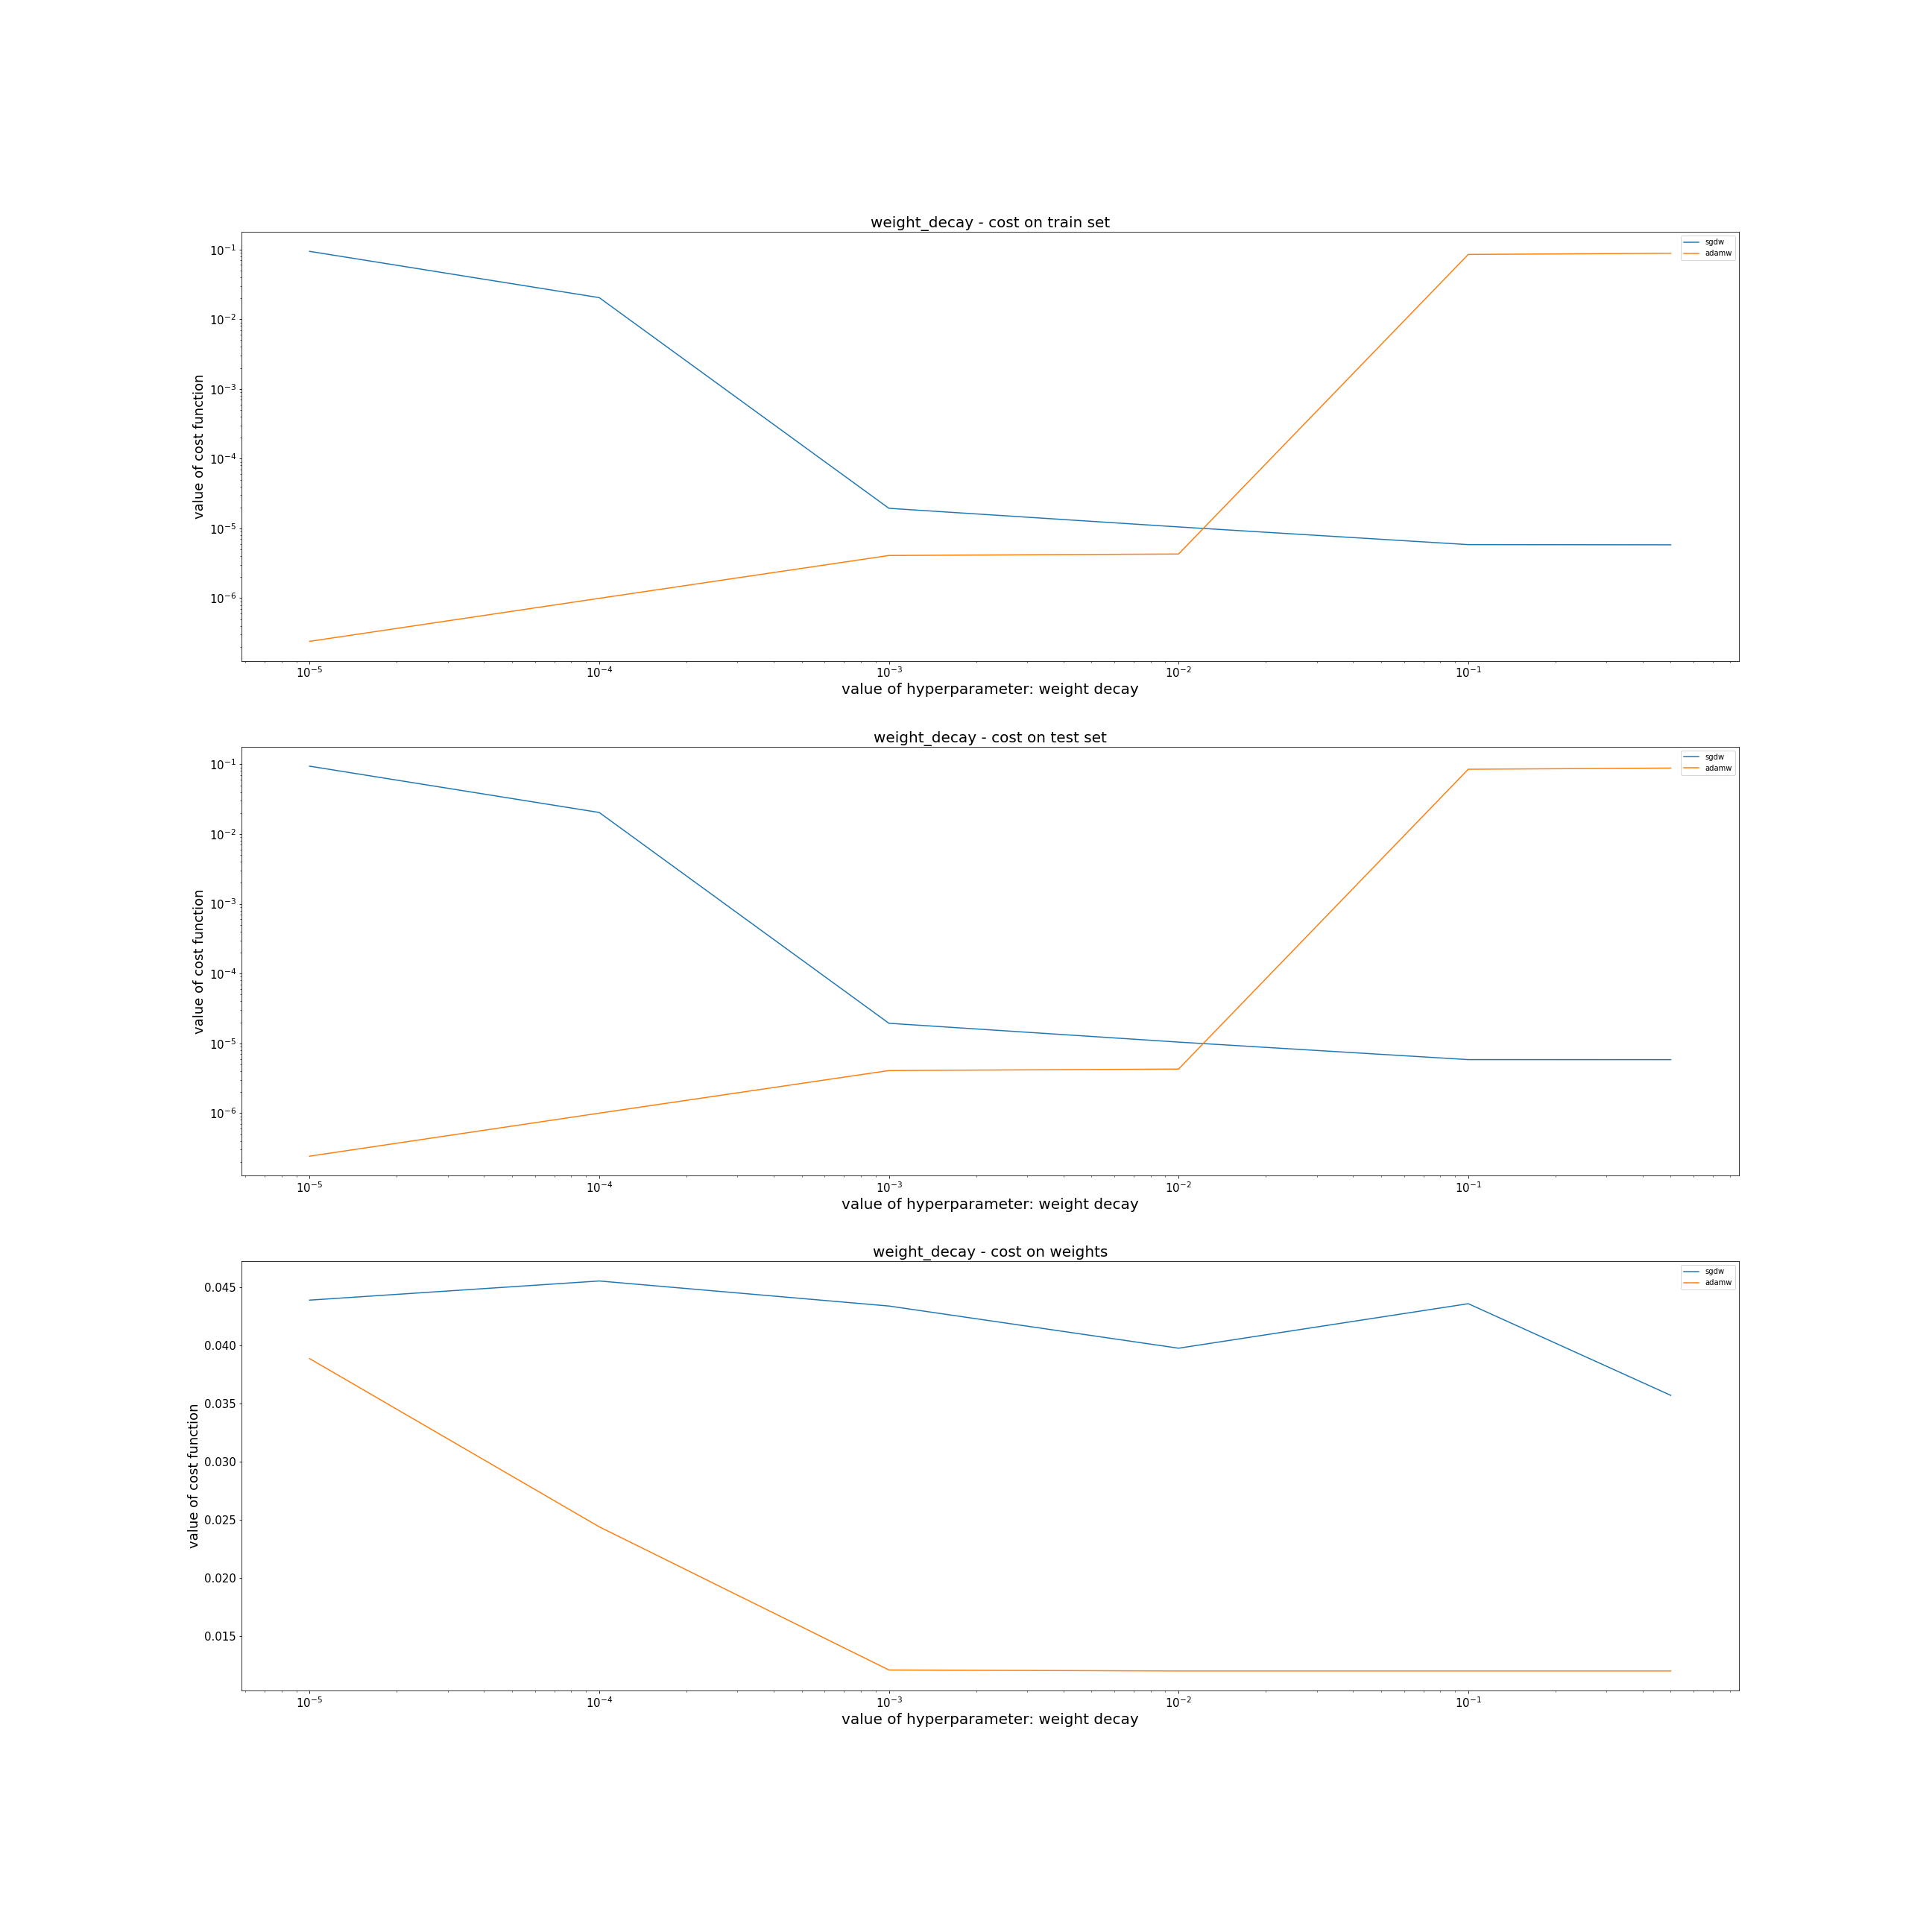
\includegraphics[width=\linewidth]{Comparision_weight_decay_ann_0.png}
	\end{subfigure}
	\label{fig:decay}
	\caption{Rezultaty nauki sieci z róznymi wartościami weight decay w optymalizatorze.}
\end{figure}
Opis testów i ich rezultatów:
\begin{enumerate}
	\item Skale na obu osiach są skalami logarytmicznymi z wyjątkiem ostatniego rysunku, gdzie na osi y jest skala liniowa.
	\item W kontekście błędu na zbiorach treningowym i testowym optymalizator SGDW osiągał najlepsze rezultaty dla weight decay większego niż 0.1, z kolei AdamW osiągał najlepsze rezultaty dla weight decay rzędu \(10^{-5}\) (W teście ann\_1 tą wartością było $10^{-4}$).
	\item Pomimo ponad stukrotnie wyższej wartości funkcji kosztu dla zestawu testowego i treningowego dla AdamW niż SGDW dla weight decay rzędu 0.1, funkcja kosztu dla wag była około 3 razy niższa dla algorytmu AdamW niż dla SGDW. W ogólności, funkcja kosztu wag była prawie stała dla SGDW (na poziomie 0.45) i malejąca dla AdamW.
\end{enumerate}

\subsubsection{Testy dropoutu}
\begin{figure}[H]
	\centering
	\begin{subfigure}[b]{1\linewidth}
		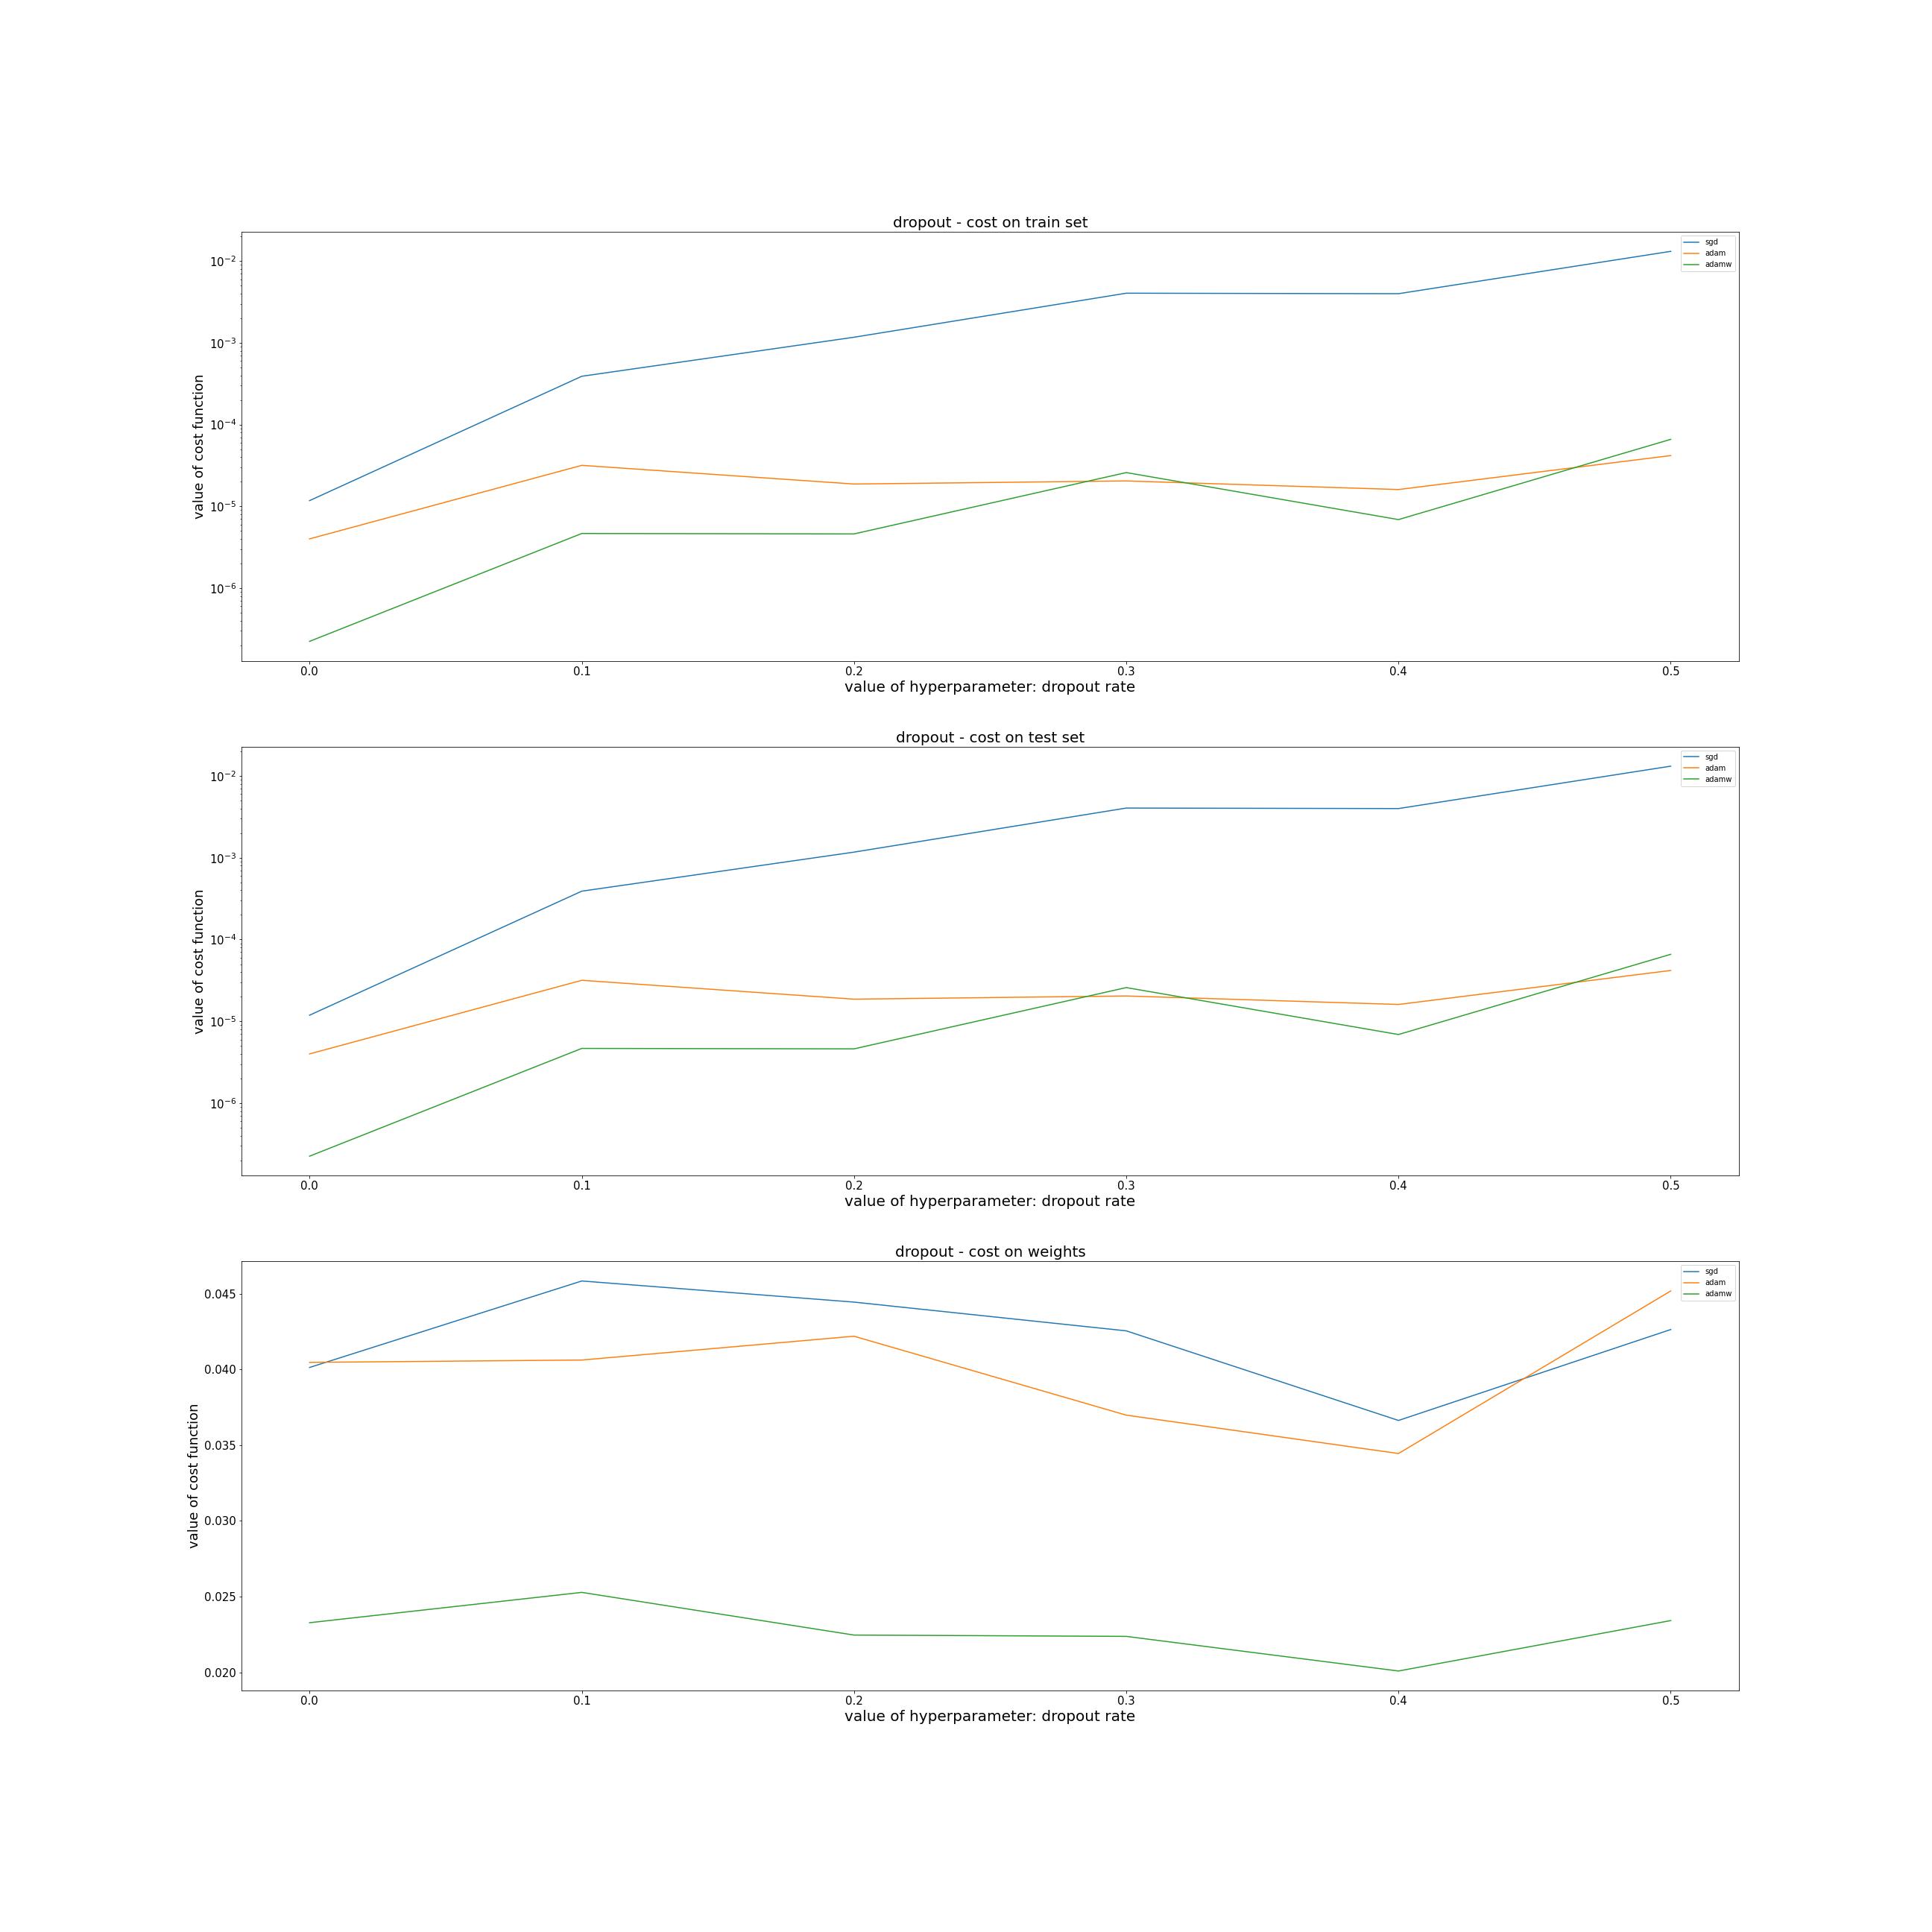
\includegraphics[width=\linewidth]{Comparision_dropout_ann_0.png}
	\end{subfigure}
	\caption{Rezultaty nauki sieci z róznymi wartościami dropout rate.}
	\label{fig:dropout}
\end{figure}
Opis testów i ich rezultatów:
\begin{enumerate}
	\item Skale na osi y są skalami logarytmicznymi z wyjątkiem ostatniego rysunku, gdzie na osi y jest skala liniowa.
	\item Wzrost dropout rate często prowadził do wyższych wartości funkcji kosztu na zestawach treningowym i testowym - może to wynikać z kilku czynników:
	\begin{enumerate}
		\item Celem dodania dropoutu jest uniknięcie przetrenowania i dostosowania się sieci neuronowej do wyników obarczonym pewnym szumem; w tych danych nie ma żadnego szumu, teoretycznie można osiągnąć funkcję kosztu równą 0 dla każdych danych.
		\item Istnienie dropoutu może penalizować próbę upodobnienia sieci testowej do wzorcowej sieci neuronowej, np. przez odrzucanie neuronów istniejących we wzorcowej sieci mających kluczowy wpływ na rezultat.
	\end{enumerate}
	\item Wszystkie 3 optymalizatory osiągały najbardziej podobną sieć neuronową do sieci wzrocowej dla $dropout\_rate=0.4$ (w teście ann\_1 tą wartością było 0.3).
	\item AdamW dopasowywał się wyraźnie lepiej do wag wzorcowej sieci niż pozostałe optymalizatory.
\end{enumerate}
\subsubsection{Uwagi ogólne}
\begin{enumerate}
	\item Najlepszą wartość funkcji kosztu dla zbioru treningowego i testowego osiągał algorytm AdamW dla batch normalization, przy $batch\_size=4$ i $momentum=0.9$ ($MSE=3.7*10^{-7}$ dla treningowego i $MSE=3.8*10^{-7}$ dla testowego).
	\item Najlepszą wartość funkcji kosztu dla wag osiągał algorytm AdamW dla batch normalization, przy $batch\_size=4$ i momentum bedącego jedną wartością z ciągu [0.5, 0.9, 0.95, 0.99] ($0.012$) dla testowego.
	\item Niewykluczone, że samo batch normalization miało mniejszy wpływ na rezultaty niż zmiana batch\_size.
	\item Optymalizator SGD osiągał gorsze wartości funkcji kosztu na zbiorach treningowym i testowym dla wszystkich testów, dla wszystkich danych.
	\item Na ogół optymalizator Adam osiągał mniej podobne wagi do sieci wzorcowej niż SGD (widoczne na wykresie \ref{fig:batch_ann} dla batch normalization). Może to wskazywać na przetrenowanie sieci przy użyciu tego optymalizatora.
	\item Regularyzacja mogła prowadzić do zmniejszenia funkcji kosztu dla porównania wag sieci wzorcowej i trenowanej, co można zauważyć na wykresie \ref{fig:dropout} (najniższy wykres pokazuje funkcję kosztu wag w zależności od dropoutu).
\end{enumerate}





\subsection{Testy drugiej sieci}\label{tit:cnn}
Rezultaty były bardzo podobne do rezultatów dla pierwszej sieci, toteż opisywane będą tylko własności niewystępujące w testach pierwszej sieci.
\subsubsection{Testy batch normalization}
\begin{figure}[h!]
	\centering
	\begin{subfigure}[b]{1\linewidth}
		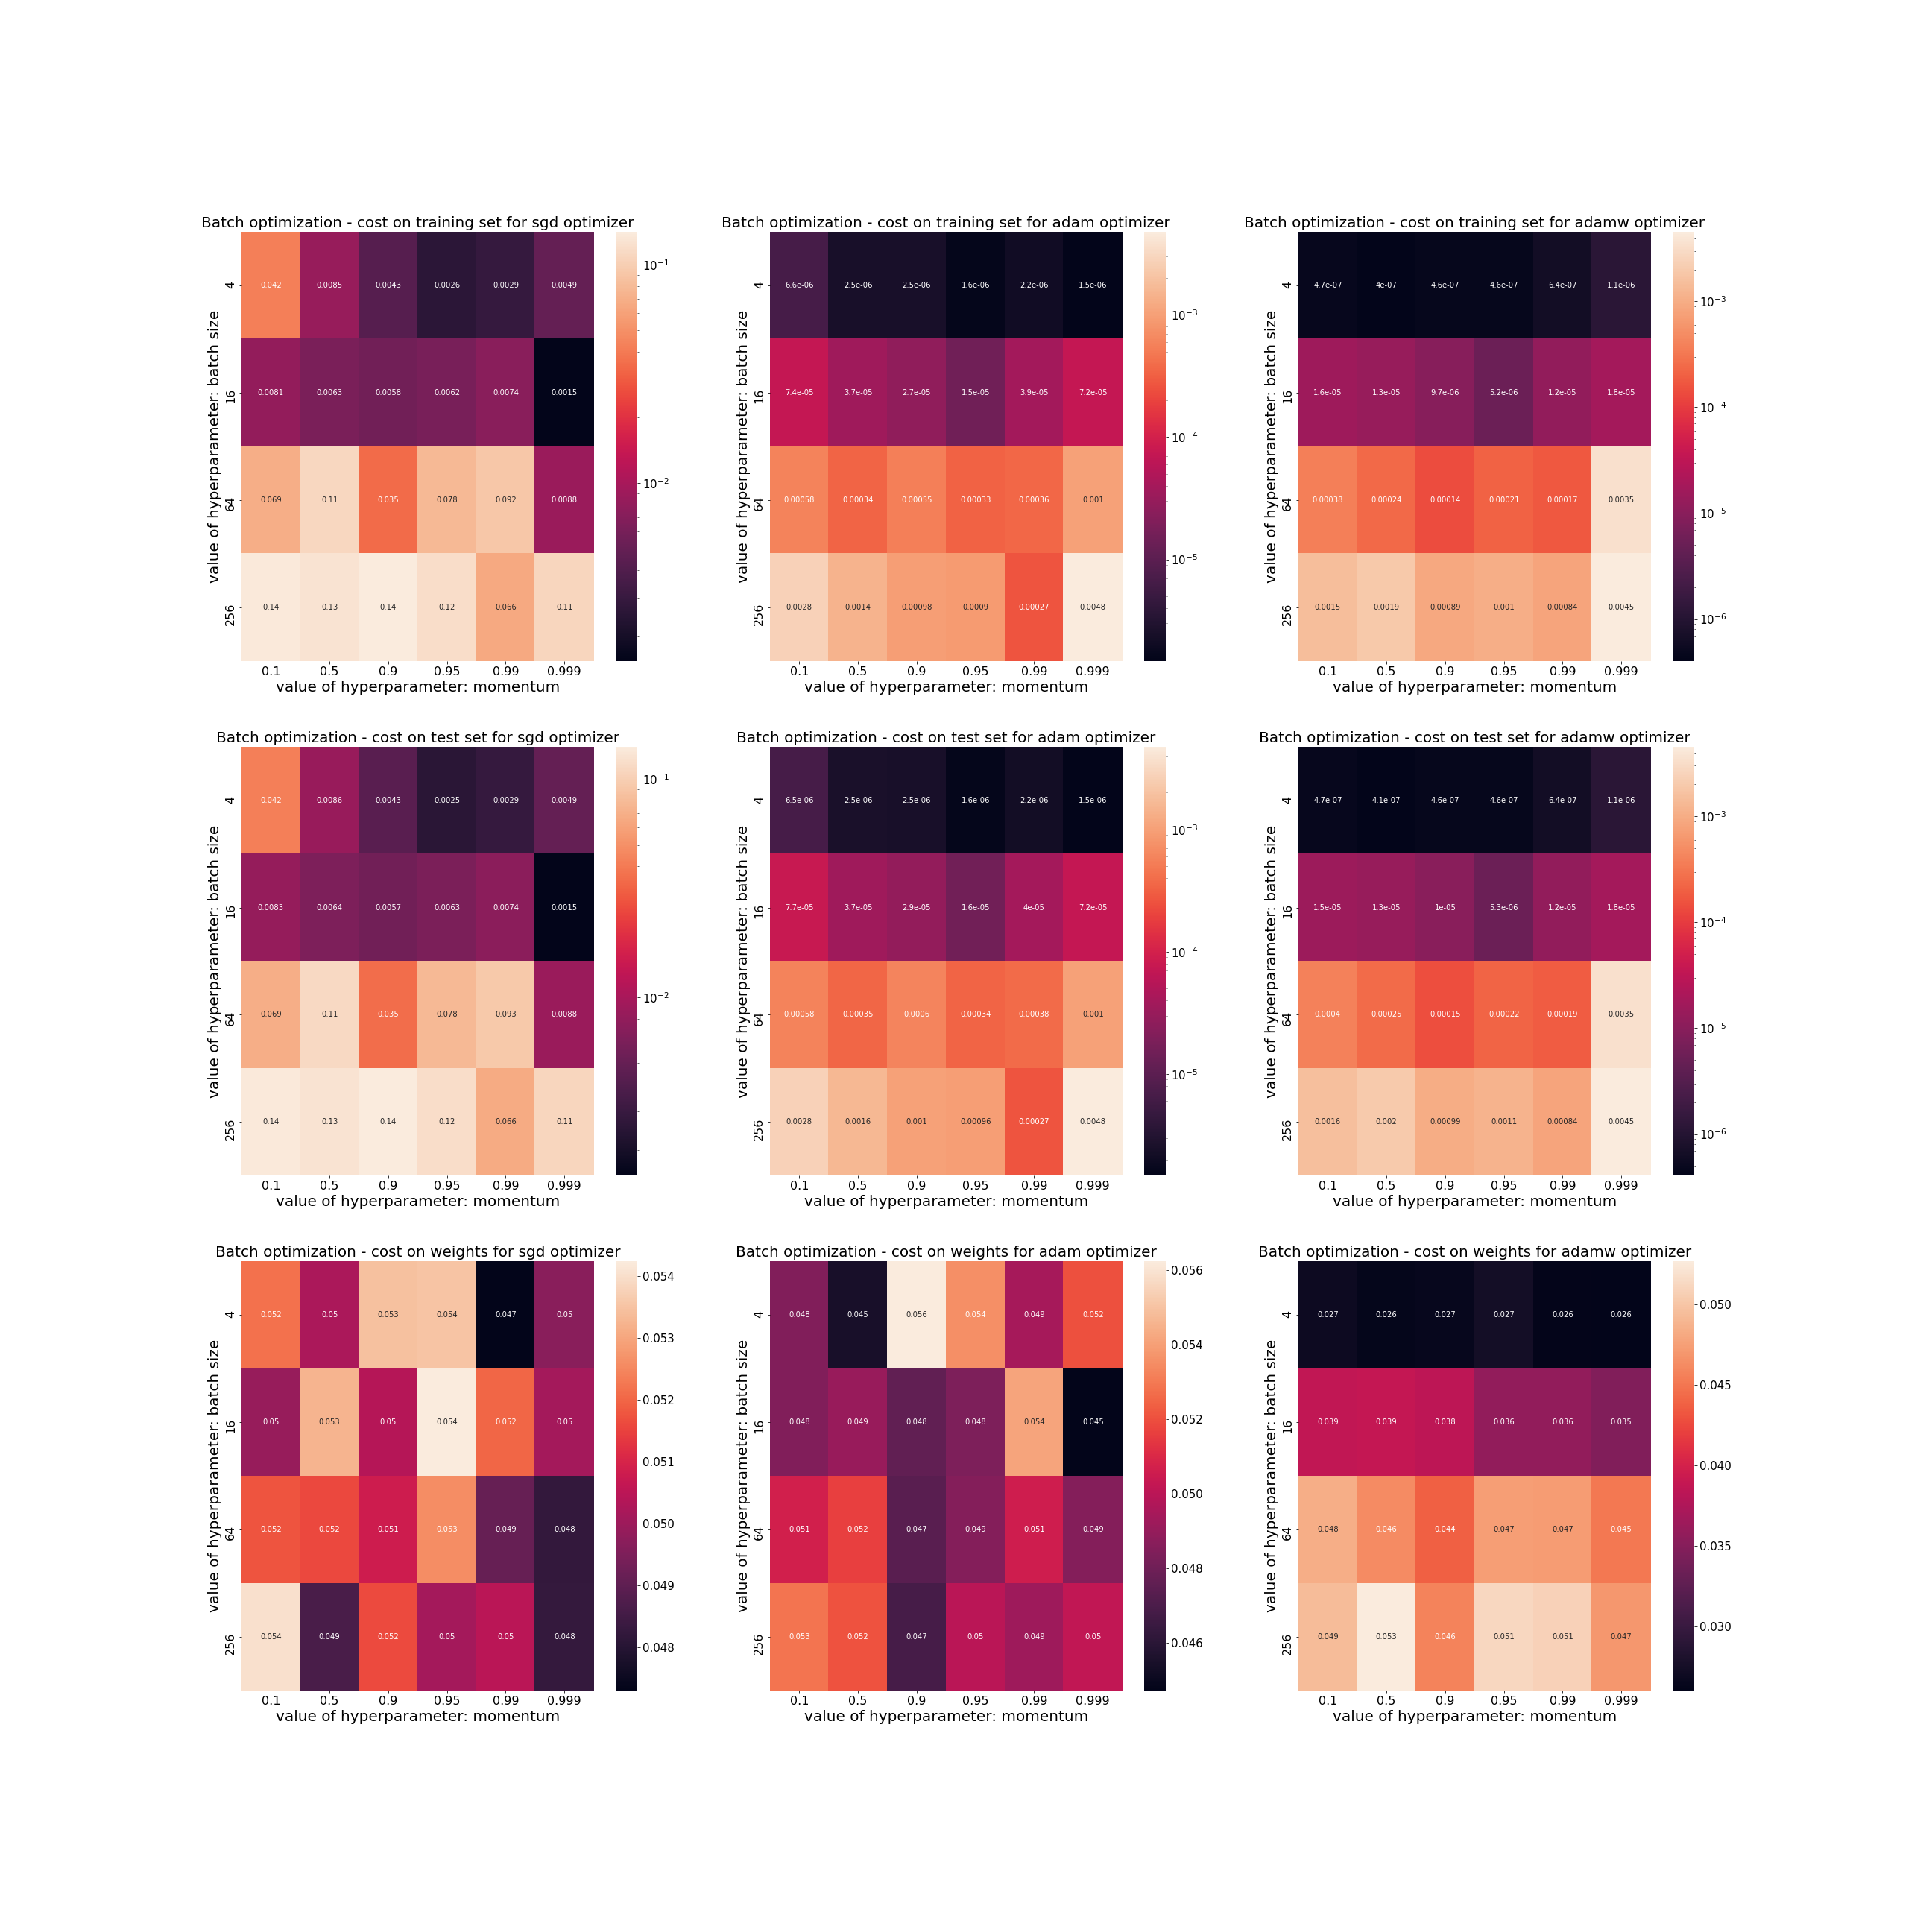
\includegraphics[width=\linewidth]{Comparision_batch_norm_conv_2.png}
	\end{subfigure}
	\label{fig:batch_cnn}
	\caption{Rezultaty nauki sieci z regularyzacją typu batch normalization}
\end{figure}
Opis testów i ich rezultatów:
\begin{enumerate}
	\item W przeciwieństwie do standardowej sieci gęstej optymalizator Adam osiąga wyraźnie lepsze rezultaty na zbiorach treningowym i testowym dla niższej wartości batch\_size.
	\item Dla optymalizatorów SGD i Adam podobieństwo wag wynikowej sieci do wag wzorcowej sieci wydaje się być niezależne od batch\_size i momentum.
\end{enumerate}

\subsubsection{Testy weight decay}
\begin{figure}[H]
	\centering
	\begin{subfigure}[b]{1\linewidth}
		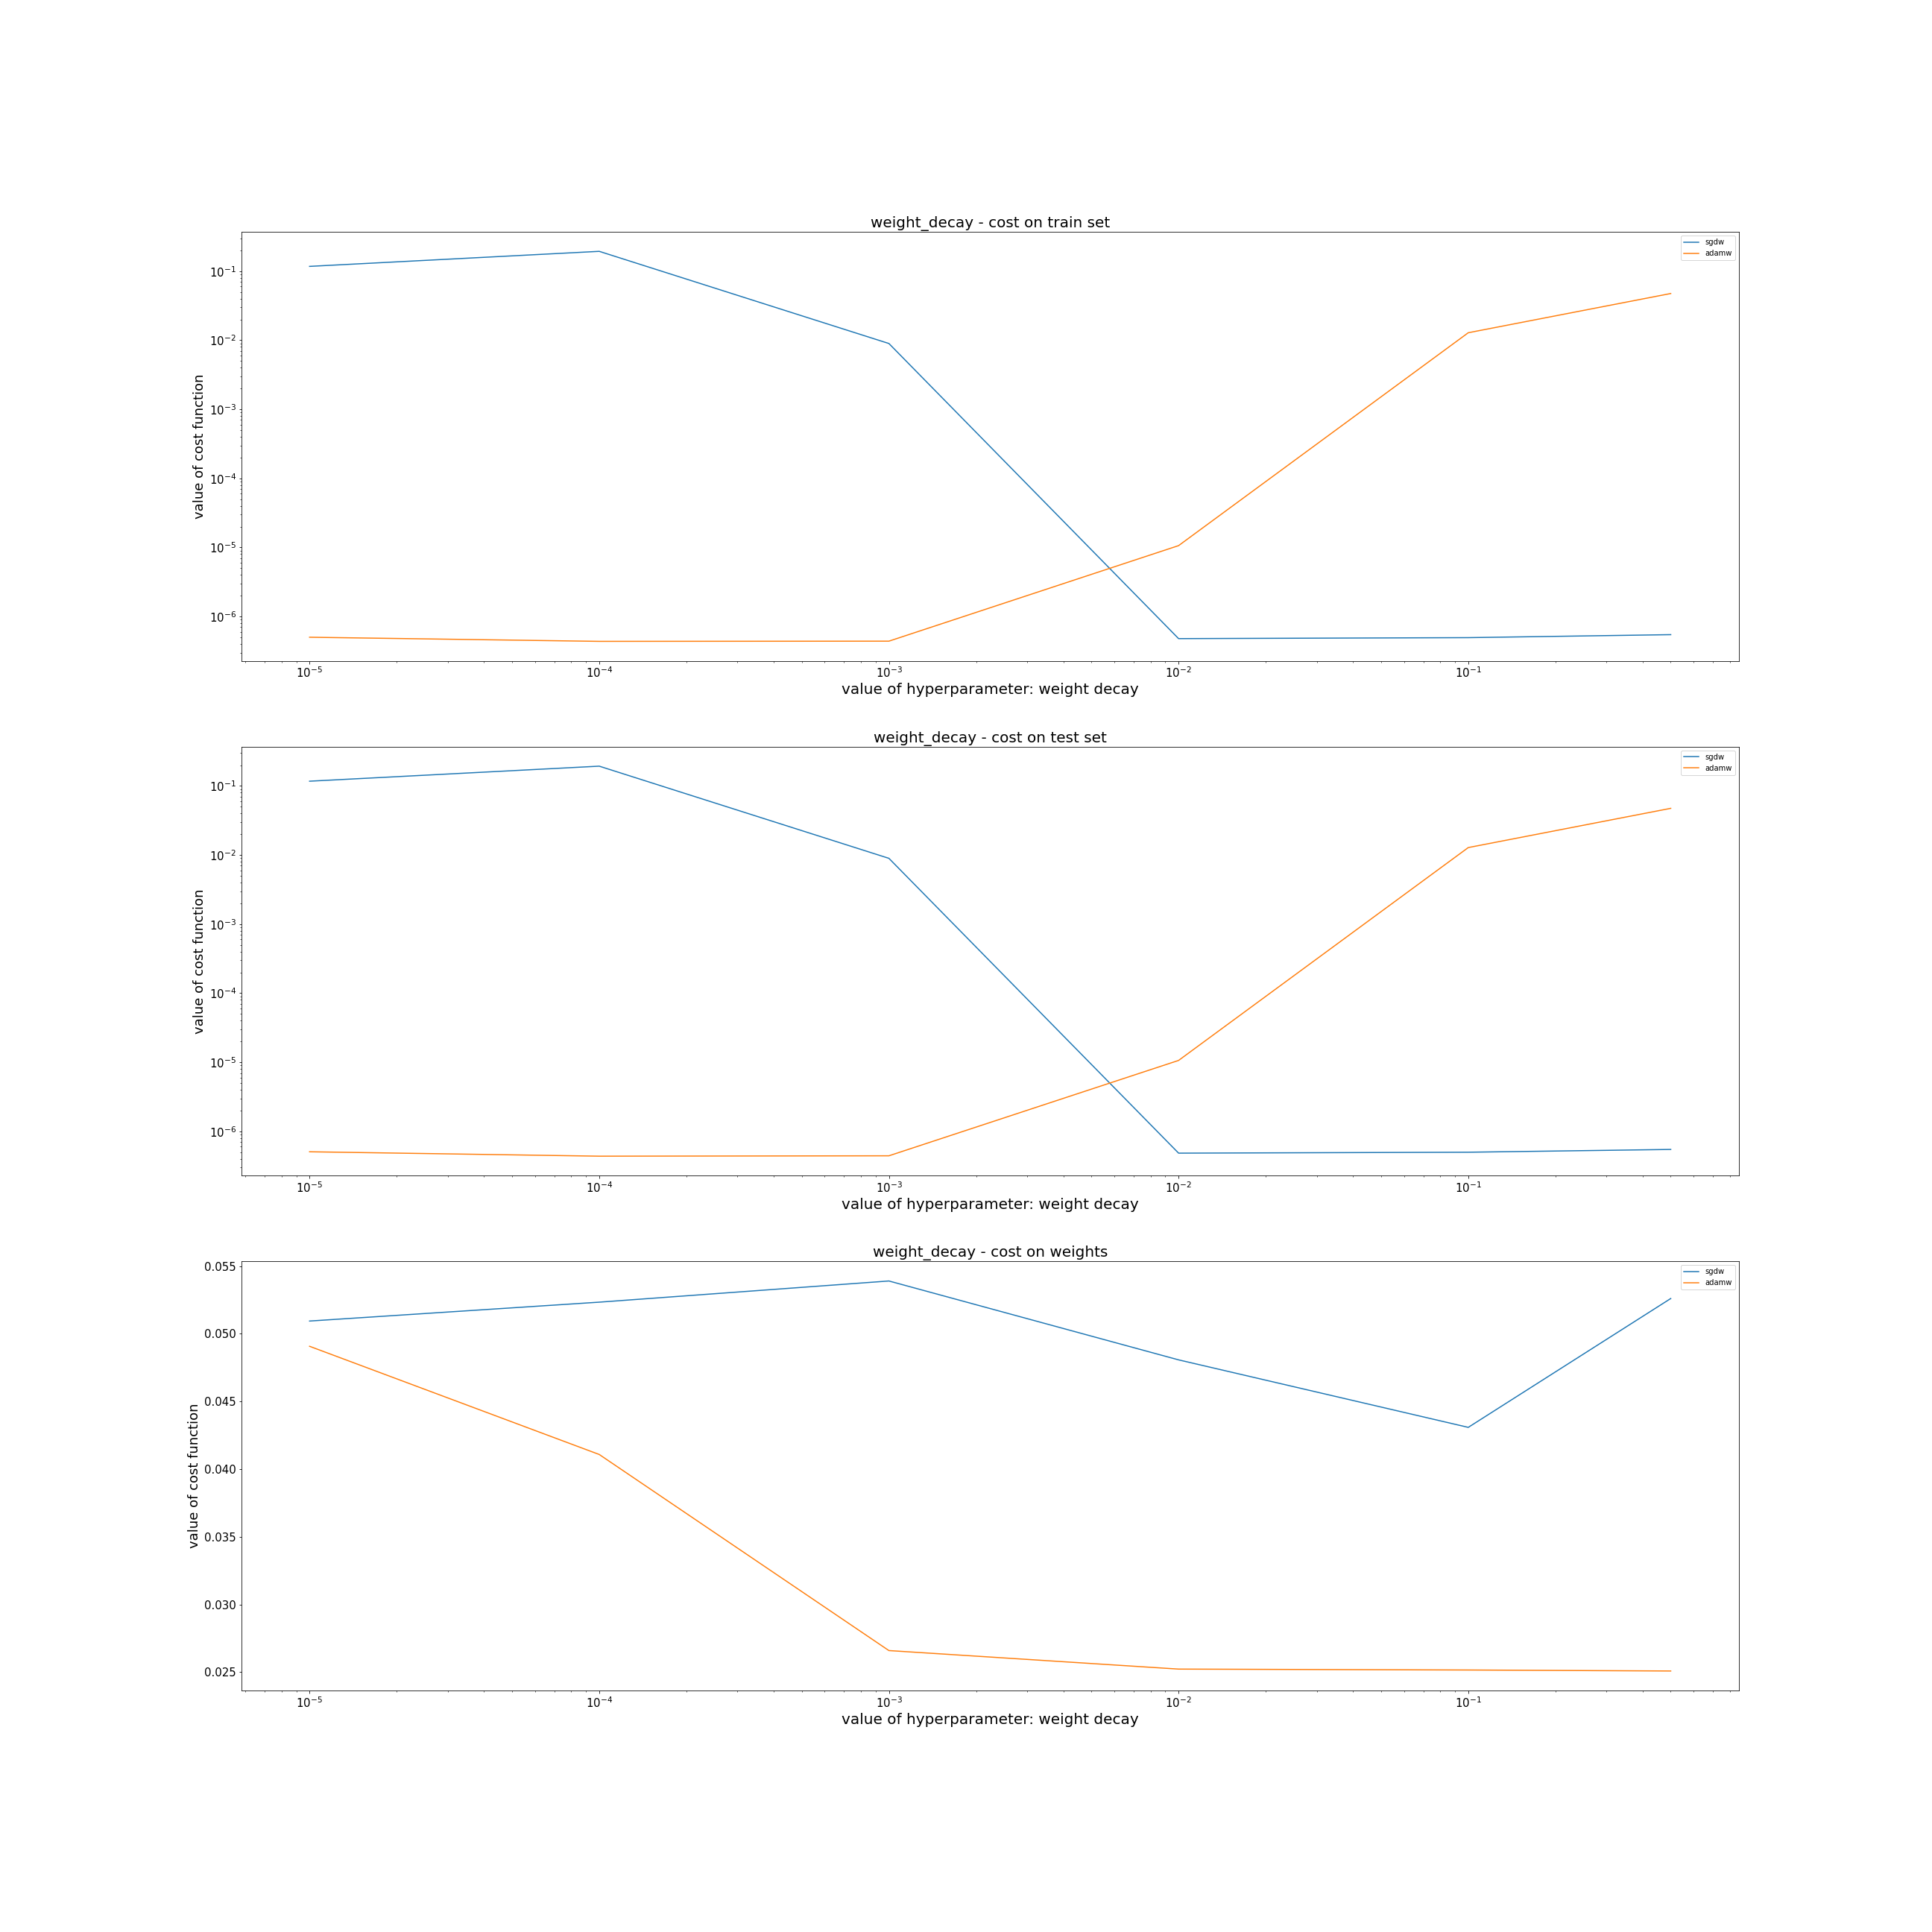
\includegraphics[width=\linewidth]{Comparision_weight_decay_conv_2.png}
	\end{subfigure}
	\label{fig:decay_cnn}
	\caption{Rezultaty nauki sieci z róznymi wartościami weight decay w optymalizatorze.}
\end{figure}
Opis testów i ich rezultatów:
\begin{enumerate}
	\item Podobny przebieg obu funkcji kosztu na zbiorze treningowym/testowym dla wszystkich przeprowadzonych testów wskazuje na to, że dla większości danych pewne wartości weight\_decay mogą (albo nawet powinny) być preferowane nad inne: dla AdamW wartości $weight\_decay \le 10^{-3}$, dla SGDW wartości $weight\_decay \ge 10^{-2}$
\end{enumerate}

\subsubsection{Testy dropoutu}
\begin{figure}[H]
	\centering
	\begin{subfigure}[b]{1\linewidth}
		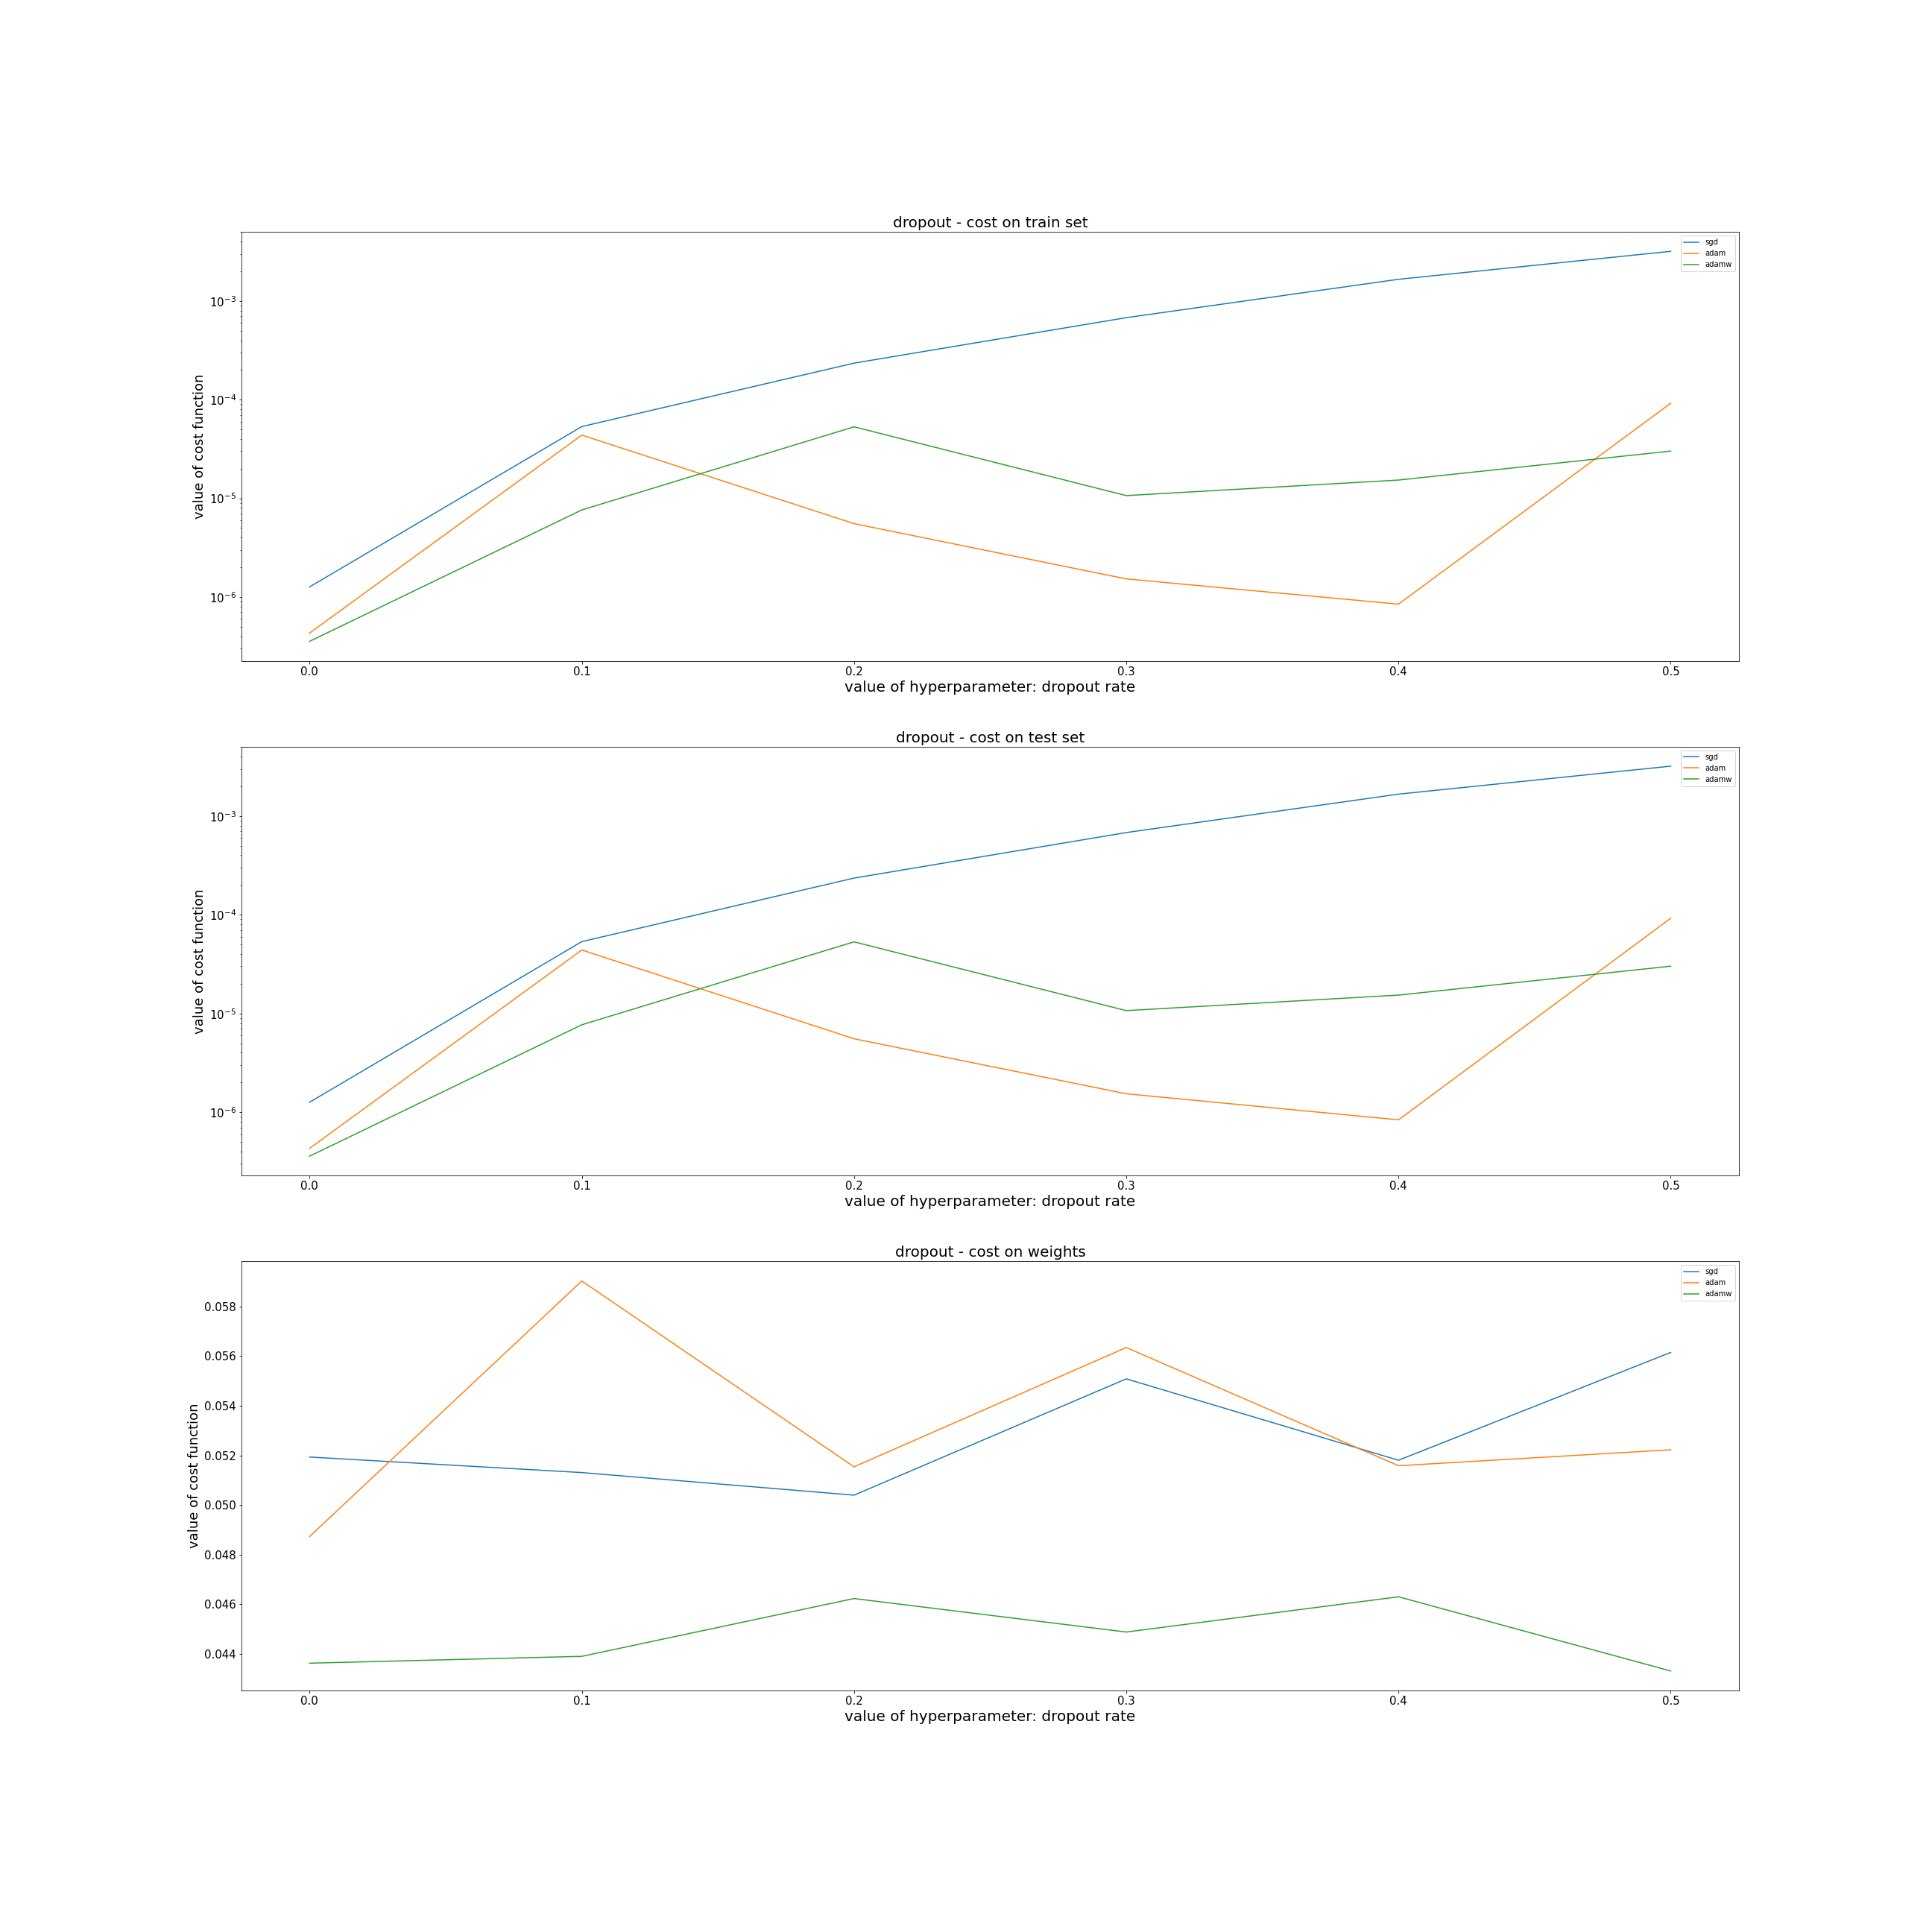
\includegraphics[width=\linewidth]{Comparision_dropout_conv_2.png}
	\end{subfigure}
	\caption{Rezultaty nauki sieci z róznymi wartościami dropout rate.}
	\label{fig:dropout_cnn}
\end{figure}
Opis testów i ich rezultatów:
\begin{enumerate}
	\item Wszystkie optymalizatory osiągały gorsze wartości funkcji kosztu dla zestawu treningowego/testowego przy istnieniu $dropout\_rate>0$
	\item Optymalizator AdamW najlepiej dopasowywał się do wag wzorcowej sieci dla $dropout\_rate=0.5$. Raczej nie byłoby zasadnym wyciągać z tego faktu dalekosiężnych konsekwencji, różnice pomiędzy tą wartością dla $dropout\_rate=0.5$ i $dropout\_rate=0$ są znikome. Wskazuje to natomiast na zasadność korzystania z tej regularyzacji jeśli celem jest dążenie do jak najbardziej podobnej sieci względem sieci wzorcowej.
\end{enumerate}
\subsubsection{Uwagi ogólne}
\begin{enumerate}
	\item Najlepszą wartość funkcji kosztu dla zbioru treningowego i testowego osiągał algorytm AdamW dla batch normalization, przy $batch\_size=4$ i $momentum=0.5$ ($MSE=4*10^{-7}$ dla treningowego i $MSE=4.1*10^{-7}$ dla testowego).
	\item Najlepszą wartość funkcji kosztu dla wag wynoszącą $0.026$ osiągał algorytm AdamW dla batch normalization, przy $batch\_size=4$ i momentum bedącego wartością z ciągu [0.99, 0.999] (Z powodu użycia innej funkcji kosztu dla wag nie ma sensu porównywać tej wartości do wartości z poprzedniej sieci).
	\item Pomimo zmiany rozkładu danych treningowych/testowych, zmniejszenia liczby ich instancji i architektury sieci, rezultaty obu testów (a także pozostałych testów, opisanych w \ref{tit:testo}) przynoszą bardzo podobne rezultaty. Tezy, które można wysnuć z tych eksperymentów zostaną sformułowane we wnioskach (\ref{tit:wniosko}).
\end{enumerate}



\subsection{Pozostałe testy - opis}\label{tit:testo}
Nazwy testów to ich symbole w folderze \textit{Comparisions}.
\begin{enumerate}
	\item Testy conv\_0 - w tych testach dla sieci konwolucyjnej w warstwach ukrytych było kolejno: 70, 50, 5 neuronów (w przedstawionych tutaj sieciach było to 100-100-5 neuronów). Funkcje aktywacji takie same, dane treningowe/testowe były generowane z rozkładu normalnego.
	\item Testy conv\_1 - w tych testach dla sieci konwolucyjnej dane treningowe/testowe były generowane z rozkładu normalnego, warstwy konwolucyjne nie miały funkcji aktywacji, poza tym test był identyczny w stosunku do opisanego w tym sprawozdaniu.
	\item Testy conv\_1 zostały opisane w tym sprawozdaniu w podrozdziale \ref{tit:cnn}.
	\item Testy ann\_0 zostały opisane w tym sprawozdaniu w podrozdziale \ref{tit:ann}.
	\item Testy ann\_1 standardowej sieci neuronowej były identyczne jak te opisane w podrozdziale \ref{tit:ann}, co za tym idzie różniły się wyłącznie wagami (i biasami). W rozdziale 2.1 przy różnicach pomiędzy tymi dwoma testami określano ten test jako 'inny test'.
\end{enumerate}

\section{Wnioski}\label{tit:wniosko}
\begin{enumerate}
	\item Optymalizator SGD zawsze osiągał gorsze rezultaty niż AdamW z weight\_decay=$10^{-4}$, ponadto nie wykonywał się znacząco szybciej niż AdamW.
	\item Wykorzystanie optymalizatora AdamW z dobrze dopasowanym weight\_decay praktycznie zawsze prowadzi do lepszych rezultatów niż wykorzystanie optymalizatora Adam w kontekście podobieństwa wag sieci neuronowych, i bardzo często w kontekście funkcji kosztu dla zbioru treningowego/testowego.
	\item Wartość weight\_decay ma bardzo duży wpływ na działanie optymalizatora, może powodować osiągnięcie nawet $10^5$ razy mniejszej funkcji kosztu niż dowolna wartość tego hiperparametru. Optymalna wartość tego hiperparametru jest zależna od algorytmu.
	\item Parametr momentum dla batch normalization na poziomie 0.95/0.99 zdaje się być odpowiedni dla testowanych optymalizatorów, jego domyślna wartość w tensorflowie wynosi 0.99.
	\item Przy używaniu batch normalization niższa wartość batch\_size niekoniecznie prowadziła do lepszej wartości funkcji kosztu pomimo dłuższego przetwarzania i większej liczby aktualizacji wag dla tej samej liczby epok (jest to widoczne dla optymalizatora SGD, wykres \ref{fig:batch_ann}).
	\item W specyficznym przypadku bez żadnego "szumu" w danych wyjściowych dropout nie prowadził do polepszenia predykcji na zbiorach treningowym i testowym, wręcz przeciwnie. Wartość dropoutu na poziomie 0.3-0.5 pozwalała natomiast czasem najlepiej dopasować się do wag sieci wzorcowej.
	\item Pomimo tego, że optymalizator Adam prawie zawsze dokonywał lepszej predykcji dla zbioru treningowego/testowego niż SGD, na ogół wagi sieci optymalizowanej przez optymalizator Adam nie były bardziej podobne do wag sieci wzorcowej niż te wynikające z użycia optymalizatora SGD; może to wskazywać na możliwość zajścia problemów dla tego optymalizatora związanych z przetrenowaniem (które w tych testach nie były widoczne, bo instancje pochodziły z tego samego rozkładu i nie było "szumu" w danych wyjściowych).
\end{enumerate}

\end{document}
